\documentclass[11pt]{article}

\usepackage[a4paper,top=1.6cm,bottom=1.6cm,left=1.9cm,right=1.9cm]{geometry}
\usepackage[spanish]{babel}
\usepackage[utf8]{inputenc}
\usepackage[T1]{fontenc}
\usepackage{graphicx}
\usepackage{booktabs}
\usepackage{array}
\usepackage{enumitem}
\usepackage{titlesec}
\usepackage{parskip}
\usepackage{hyperref}
\usepackage{caption}

\setlength{\parindent}{0pt}
\setlength{\parskip}{4pt}

\titlespacing*{\section}{0pt}{8pt}{4pt}
\titlespacing*{\subsection}{0pt}{6pt}{3pt}
\titleformat{\section}{\normalfont\bfseries\large}{\thesection.}{0.5em}{}
\titleformat{\subsection}{\normalfont\bfseries}{\thesubsection}{0.5em}{}

\captionsetup{font=small,labelfont=bf,justification=centering}

\hypersetup{colorlinks=true, urlcolor=blue, linkcolor=black}

\pagenumbering{gobble}

\begin{document}

% ---------- Encabezado ----------
\begin{center}
  
\includegraphics[width=2.1cm]{assets/uvg_logo.png}\\[4pt]
  {\bfseries UNIVERSIDAD DEL VALLE DE GUATEMALA}\\
  {\bfseries CC3092 -- Deep Learning y Sistemas Inteligentes}\\[2pt]
  {\large\bfseries Laboratorio \#5: Agentes en el Arcade Learning Environment (ALE): Space Invaders}\\[4pt]
  Pedro Rub\'en Avila Cofi\~no, \#23089 \\
  Guatemala, 13 de septiembre de 2026
\end{center}

\vspace{2pt}
\hrule
\vspace{6pt}

% ================= 1. ALE =================
\section{El Arcade Learning Environment (ALE)}

El \textbf{Arcade Learning Environment (ALE)} es un framework de investigaci\'on que expone m\'as
de 100 juegos originales de \textbf{Atari 2600} como entornos de aprendizaje por refuerzo con una
interfaz program\'atica uniforme (observaci\'on, acci\'on, recompensa). Resuelve el problema de no
contar con un banco est\'andar de entornos de percepci\'on-y-control de dificultad realista: antes
de ALE, evaluar agentes de RL en tareas con observaciones ricas (im\'agenes) y din\'amicas
complejas requer\'ia construir simuladores ad-hoc. ALE se apoya internamente en \textbf{Stella},
un emulador de c\'odigo abierto del hardware original del Atari 2600 (el mismo binario \texttt{.bin}
de la ROM corre sin modificaciones); ALE a\~nade sobre Stella la extracci\'on de frames, el
c\'omputo de la recompensa a partir de la memoria del juego y una API tipo Gym para controlar el
emulador paso a paso.

Gymnasium expone cada juego bajo el espacio de nombres \texttt{ALE/<Juego>-v5} (p. ej.
\texttt{ALE/SpaceInvaders-v5}), que usa por defecto observaciones de imagen RGB e internamente fija
un \texttt{frameskip} estoc\'astico y una peque\~na probabilidad de repetir la \'ultima acci\'on
(\texttt{repeat\_action\_probability}$=0.25$) para introducir estocasticidad y evitar que un agente
memorice una secuencia fija de acciones. La variante con sufijo \texttt{-ram} (p. ej.
\texttt{ALE/SpaceInvaders-ram-v5}) usa exactamente el mismo emulador y la misma din\'amica, pero
sustituye la observaci\'on de imagen por los 128 bytes de memoria de la consola. Otros
par\'ametros de \texttt{gym.make} permiten ajustar este comportamiento: \texttt{frameskip} controla
cu\'antos frames de emulaci\'on se ejecutan (y se repite la misma acci\'on) por cada llamada a
\texttt{step()}; \texttt{repeat\_action\_probability} controla la estocasticidad ``sticky actions'';
y \texttt{full\_action\_space} determina si se expone el conjunto completo de 18 acciones del
joystick Atari o solo el subconjunto m\'inimo relevante para el juego (6 en Space Invaders).

El \textbf{frame skipping} es central en los entornos Atari porque el emulador corre internamente a
60 frames por segundo, una resoluci\'on temporal mucho m\'as fina de la que necesita un agente de
decisi\'on: repetir cada acci\'on durante $k$ frames (t\'ipicamente $k=4$) reduce en ese mismo
factor el n\'umero de decisiones -y de pasos de entrenamiento- necesarias para jugar un episodio
completo, acelerando dr\'asticamente tanto la simulaci\'on como el aprendizaje, sin perder
capacidad de control real (las din\'amicas relevantes del juego cambian poco en 4 frames = $1/15$s).

\textbf{Space Invaders} es un juego de disparos de 1978 en el que el jugador controla un ca\~n\'on
en la parte inferior de la pantalla y debe destruir una formaci\'on de alien\'igenas que descienden
progresivamente, evitando sus disparos y protegi\'endose tras refugios destructibles; el juego
termina cuando el ca\~n\'on pierde sus 3 vidas o los alien\'igenas llegan al fondo de la pantalla.
En ALE, el \texttt{reward} de cada paso corresponde directamente al incremento del marcador
(\textit{score}) del juego original en esos frames (p. ej. destruir un alien\'igena de la fila
superior otorga m\'as puntos que uno de la fila inferior), sin normalizar ni recortar por defecto.

% ================= 2. Observacion / accion =================
\section{Espacios de observaci\'on y acci\'on en entornos Atari}

Por defecto, \texttt{ALE/SpaceInvaders-v5} expone una observaci\'on \texttt{Box(0, 255, (210, 160,
3), uint8)}: un frame RGB completo de $210\times160$ p\'ixeles. Esto contrasta fuertemente con
\texttt{CartPole-v1} (visto en el laboratorio anterior), cuya observaci\'on es un vector
\texttt{Box(4,)} de bajo nivel (posici\'on y velocidad del carro, \'angulo y velocidad angular del
poste) ya calculado por el simulador. Trabajar con im\'agenes en vez de vectores de bajo nivel
implica que el agente debe aprender por s\'i mismo a extraer las caracter\'isticas relevantes
(posiciones, velocidades) a partir de p\'ixeles crudos -un problema de percepci\'on adem\'as de uno
de control-, lo que multiplica la dimensionalidad de entrada ($210\times160\times3 = 100{,}800$
valores frente a 4) y hace casi obligatorio el uso de redes convolucionales y de m\'as datos/tiempo
de entrenamiento.

La variante \texttt{obs\_type='ram'} expone directamente los 128 bytes de memoria de trabajo de la
consola Atari 2600 (posiciones de sprites, marcador, vidas, etc., codificados por el propio juego).
Es preferible sobre la imagen cuando se quiere reducir dr\'asticamente el costo computacional y la
dimensionalidad de entrada (128 valores en vez de $\sim$100K) y se est\'a dispuesto a perder
interpretabilidad, ya que el significado de cada byte no est\'a documentado y var\'ia por juego.

El espacio de acci\'on de Space Invaders es \texttt{Discrete(6)}, con significados
\texttt{NOOP} (no hacer nada), \texttt{FIRE} (disparar), \texttt{RIGHT}/\texttt{LEFT} (mover el
ca\~n\'on) y \texttt{RIGHTFIRE}/\texttt{LEFTFIRE} (moverse y disparar en el mismo paso); este es el
subconjunto \textit{minimal} relevante para el juego (con \texttt{full\_action\_space=True} se
expondr\'ian las 18 acciones del joystick completo del Atari 2600).

El wrapper \texttt{AtariPreprocessing} de Gymnasium encapsula el preprocesamiento est\'andar usado
en la literatura de DQN: convierte la imagen a escala de grises, la redimensiona a $84\times84$,
aplica \textit{frame skipping} internamente (tomando el m\'aximo entre los \'ultimos dos frames
para evitar parpadeo de sprites) y opcionalmente recorta la recompensa a $\{-1,0,1\}$.
\texttt{FrameStackObservation} (antes \texttt{FrameStack}) apila los \'ultimos $n$ frames
preprocesados en un solo tensor de observaci\'on; se usa junto con \texttt{AtariPreprocessing}
porque un \'unico frame est\'atico no contiene informaci\'on de movimiento (direcci\'on/velocidad
de sprites), algo indispensable para que una pol\'itica pueda decidir bien.

% ================= 3. Modulo =================
\section{M\'odulo de desarrollo: funciones para interactuar con ALE}

Se implement\'o el m\'odulo \texttt{scripts/ale\_utils.py} con las cinco funciones reutilizables
solicitadas, probadas end-to-end en el notebook \texttt{notebook/Lab05\_ALE\_SpaceInvaders.ipynb}:

\begin{itemize}[leftmargin=1.4em, itemsep=1pt, topsep=2pt]
  \item \textbf{\texttt{crear\_entorno(nombre\_entorno, video\_folder=None, episode\_trigger=None,
  name\_prefix, **kwargs)}}: crea el entorno con \texttt{gym.make}; si se pasa
  \texttt{video\_folder}, fuerza \texttt{render\_mode='rgb\_array'} y envuelve el entorno con
  \texttt{gymnasium.wrappers.RecordVideo}. Es gen\'erica: funciona igual para
  \texttt{ALE/SpaceInvaders-v5} que para cualquier otro entorno de Gymnasium.
  \item \textbf{\texttt{agente\_aleatorio(observation, env)}}: retorna
  \texttt{env.action\_space.sample()}, usado como \textit{baseline} sin entrenamiento.
  \item \textbf{\texttt{agente\_regla\_simple(observation, env)}}: pol\'itica fija sin
  entrenamiento que alterna bloques de 10 pasos disparando y movi\'endose a la derecha
  (\texttt{RIGHTFIRE}) y a la izquierda (\texttt{LEFTFIRE}); si el entorno no expone esas acciones
  (otro juego/entorno), cae de vuelta al muestreo aleatorio.
  \item \textbf{\texttt{ejecutar\_episodio(env, funcion\_agente, max\_steps=10000)}}: corre un
  episodio hasta \texttt{terminated}/\texttt{truncated} o \texttt{max\_steps}, retornando pasos y
  recompensa total acumulada.
  \item \textbf{\texttt{generar\_video\_agente(nombre\_entorno, funcion\_agente, video\_folder,
  name\_prefix, n\_episodios=1)}}: combina las anteriores, graba \texttt{n\_episodios} con
  \texttt{RecordVideo}, cierra el entorno (\texttt{env.close()}, indispensable para que el
  \texttt{.mp4} se escriba a disco) y retorna las rutas de video junto con las m\'etricas de cada
  episodio.
\end{itemize}

Un detalle de infraestructura no trivial: el paquete \texttt{ale-py} de nixpkgs (usado en el
\texttt{flake.nix} del proyecto) no incluye los binarios de ROM por pol\'itica de empaquetado. El
m\'odulo fija la variable \texttt{ALE\_ROMS\_DIR} apuntando a \texttt{assets/roms/}, donde se
distribuye \texttt{space\_invaders.bin} (obtenido del paquete oficial \texttt{ale-py} de PyPI, cuyas
ROMs est\'an licenciadas para uso libre/investigaci\'on desde ALE~0.8.0, y verificado contra el hash
MD5 que el propio \texttt{ale-py} espera), de modo que el entorno se pueda crear sin pasos manuales
adicionales.

\subsection*{Resultados}

Usando \texttt{ejecutar\_episodio} directamente (sin grabaci\'on) se corrieron 5 episodios de cada
agente sobre \texttt{ALE/SpaceInvaders-v5}:

\begin{center}
\small
\begin{tabular}{lrr}
\toprule
\textbf{Agente} & \textbf{Pasos promedio (5 eps)} & \textbf{Return promedio (5 eps)} \\
\midrule
\texttt{agente\_aleatorio} & 605.6 & 224.0 \\
\texttt{agente\_regla\_simple} & 374.2 & 75.0 \\
\bottomrule
\end{tabular}
\end{center}

\begin{figure}[h]
  \centering
  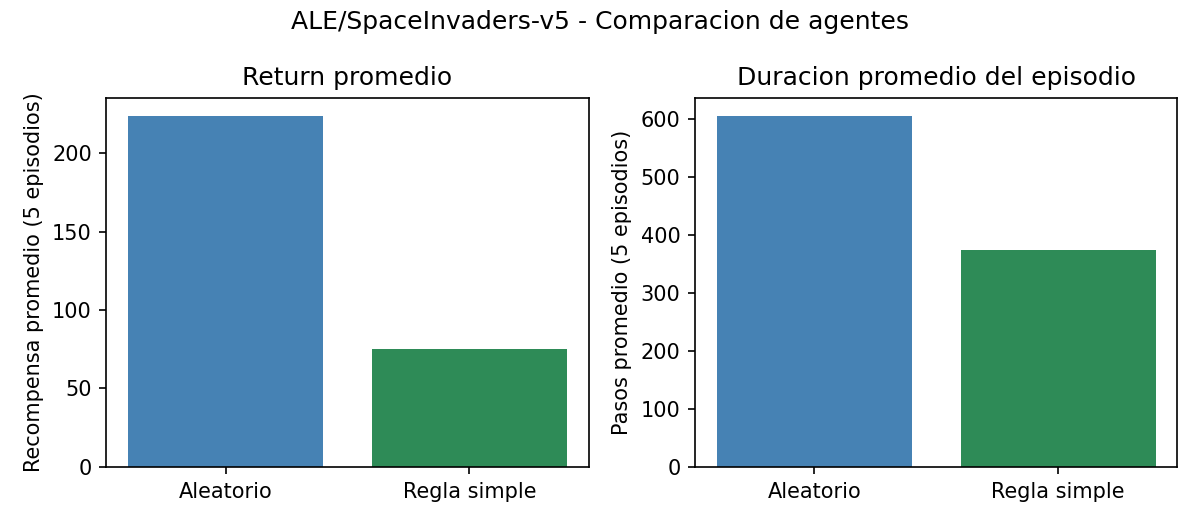
\includegraphics[width=0.78\linewidth]{fig_spaceinvaders_comparison.png}
  \caption{Return y duraci\'on promedio (5 episodios) del agente aleatorio vs. el agente de regla simple.}
\end{figure}

El agente aleatorio obtuvo, en promedio, mayor recompensa y episodios m\'as largos que la regla
fija de disparo/movimiento alterno; esto es consistente con que Space Invaders recompensa
principalmente impactar alien\'igenas en posiciones variadas, algo que el muestreo aleatorio cubre
mejor en pocos episodios que una regla determinista y repetitiva, la cual adem\'as puede quedar
``atrapada'' disparando siempre hacia el mismo lado de la formaci\'on.

Con \texttt{generar\_video\_agente} se gener\'o el video entregable de 1 episodio completo del
agente aleatorio (\texttt{entregables/videos/space-invaders-aleatorio-episode-0.mp4}: 373 pasos,
return de 105.0), y adicionalmente uno del agente de regla simple
(\texttt{space-invaders-regla-simple-episode-0.mp4}: 480 pasos, return de 155.0) a modo de
comparaci\'on visual. Ambos videos, junto con las m\'etricas impresas por episodio, quedan
documentados en el notebook y en la carpeta \texttt{entregables/videos/}.

\end{document}
